\chapter{Introduction}
\label{chap:intro}
Traditionally, people rely single supercomputer to calculate data or deploy their companies' application. Nowadays, cloud computing has been use wildly. People would like to use a lot of normal computers that gather them into a cluster to replace a supercomputer. More and more companies build their data centres or use cloud platforms to construct their business application.
However, the more computers we have, the more power consumption problem we have to solve. At the same time, to make sure every computers' process in the cluster are alive, high availability becomes a more important role in cloud computing.

Virtualization is a popular technology that is used wildly on cloud computing,  including virtual operating system, computer hardware platforms, storage device and computer network resources.
Virtual machine is a technology to emulate a particular computer like a real computer. It can partition a physical machine resource, such as CPU, memory, storage, and network.
A hypervisor uses execution to manage and share host physical machine hardware, it allows many different virtual machines isolated from each other.

Container is operating system level virtualization which runs as an isolated process in userspace on the host operating system and shares the same operation system kernel with other containers.
It provides kernel namespace such as PID, IPC, network, mount, and user namespace to isolate each container environment to host operation system.
In order to control hardware resource like CPU, memory, network, and disk I/O, container uses cgroups to limit each container resources.
Container doesn't have hypervisor to isolate with host operating system, therefore, it can offer better performance than virtual machine. It already has many software to control container, like LXC \cite{helsley2009lxc}, LXD, Open VZ, For now, Docker \cite{Docker} is the most popular container engine. The Virtual Machine and Container architecture is shown as Fig \ref{fig:VM_vs_container}.

\begin{figure}[h]
\begin{center}
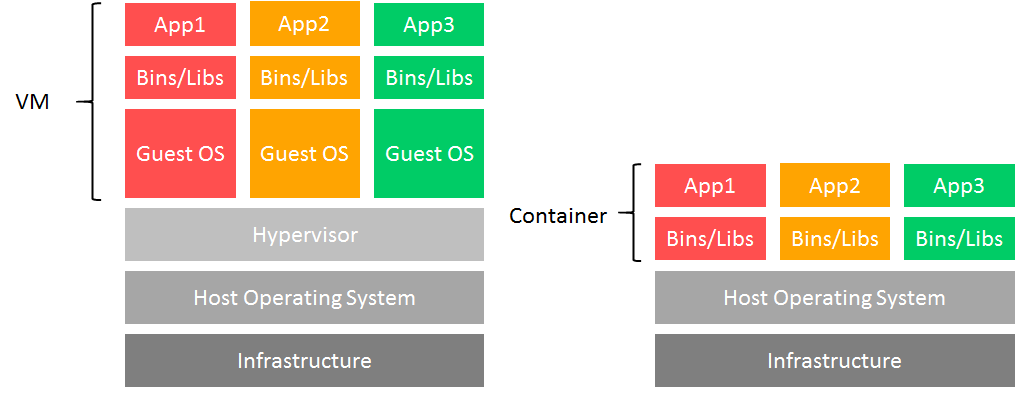
\includegraphics[width=15cm]{figure/VM_vs_container.png}
\end{center}
\caption{Virtual Machine and Container architecture}
\label{fig:VM_vs_container}
\end{figure}

Checkpoint and restoration can freeze a running process state and save process information to checkpoint images. User can use these checkpoint image files to restore the process which user want to restore the process state. These features can be used to dump checkpoint and restore containers because each containers are processes in the host operating system.

In this paper, we choose container but not Virtual Machine to do migration between two host machines, because container need less disk storage and less network transport resources. We not only use checkpoint and restoration to migrate the containers between two physical computers but also migrate the containers in the Docker cluster.
There are many Docker cluster software, like Docker Swarm, Google Kubernetes, Apache Mesos, etc. We choose Docker Swarm because it support native Docker API, and Docker usage habit. We don't need to learn the other Docker cluster software.
Moreover, we improve high availability and rescheduling feature in Docker Swarm using checkpoint and restoration than keep versions of container checkpoint images in remote storage server that whenever computer are fail, Docker Swarm manager will restore the containers from the checkpoint images.
